

Prima di entrare nel merito delle soluzioni e problemi affrontati, descriverò in questo capitolo i concetti e
gli strumenti base di iOS che mi sono stati utili nella progettazione e implementazione finale dell'applicazione.
In particolare descriverò per prima cosa i componenti iOS che permettono di definire la navigazione
all'interno di un'applicazione iOS. In seguito descriverò un framework nativo di iOS atto a creare animazioni
fisiche, l'utilizzo della UIWindow e le tipologie di gestione del touch screen.

\section{Navigazione standard}

Un'applicazione iOS è un insieme di \textbf{UIViewController}\cite{viewcontroller} diversi che 
regolano ogni aspetto della lora vista.

Qualsiasi applicazione ha infatti un rootViewController, ossia un ViewController di partenza
che sarà il primo elemento attivo sulla \textbf{UIWindow}.

Ogni applicazione può avere degli \textbf{UINavigationController}\cite{navigationcontroller},
ossia dei contenitori di \textbf{UIViewController} che vengono
utilizzati per mantenere lo stack di navigazione e gestire la transizioni tra due UIViewController.

Nella figura~\ref{fig:1} si nota come un NavigationController gestisce un'array di ViewController e una sola 
navigation bar. \\
% In iOS sono infatti innate molte animazioni di navigazione che è utile sfruttare, piuttosto di creare 
% componenti custom poi difficili da rendere interattivi.\\

\begin{minipage}{\linewidth}
    \centering
    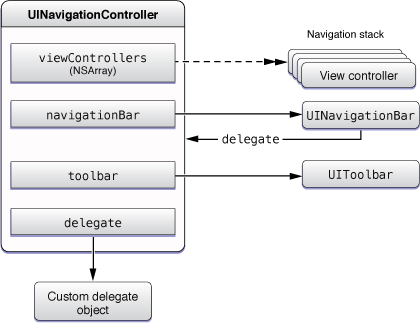
\includegraphics[width=5cm]{navigation}
    \captionof{figure}{Navigation controller scheme}
    \label{fig:1}
\end{minipage}

\subsection{Tipologie di navigazione}\label{sec:navigation}

Esistono tre tipologie base di navigazione:

\begin{enumerate}
    \item{\textbf{Push}: un UIViewController figlio di un NavigationController può rendere
    visibile un altro ViewController attraverso la funzione 
    "pushViewController" di un Navigation controller. Ogni UIViewController ha
    infatti un puntatore al UINavigationController genitore, che gestisce la navigazione.

    \par
    \begin{minipage}{\linewidth}
        \centering
        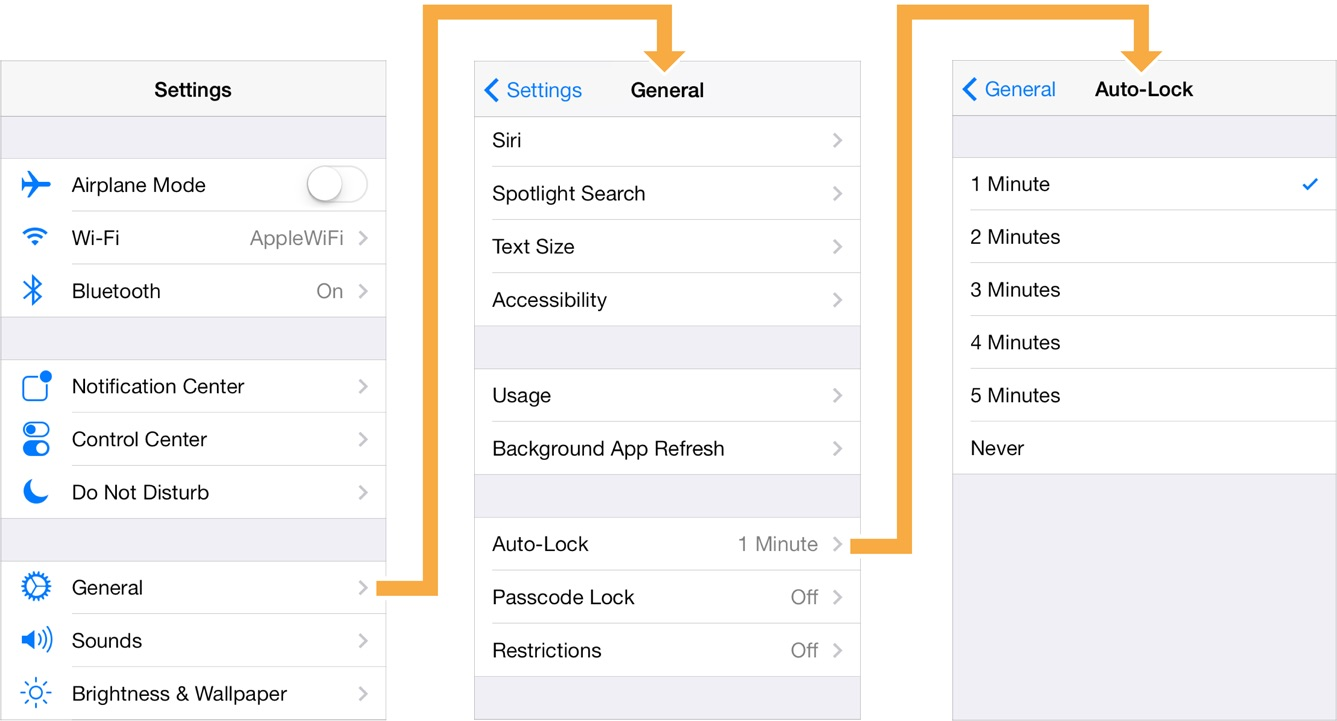
\includegraphics[width=10cm]{push}
        \captionof{figure}{Presantazione di un ViewController tramite push}
        \label{fig:2}
    \end{minipage}
    }
    \item{ \textbf{Modal}: un ViewController può presentare un altro ViewController senza necessariamente avere un 
        Navigation Controller. L'animazione standard è dal basso verso l'alto come in figura~\ref{fig:3}. La navigazione modale viene
        usata solitamente per la presentazione di task che richiedono una sola operazione oppure per rendere evidente un cambio del contesto precedente.
        \par
        \begin{minipage}{\linewidth}
            \centering
            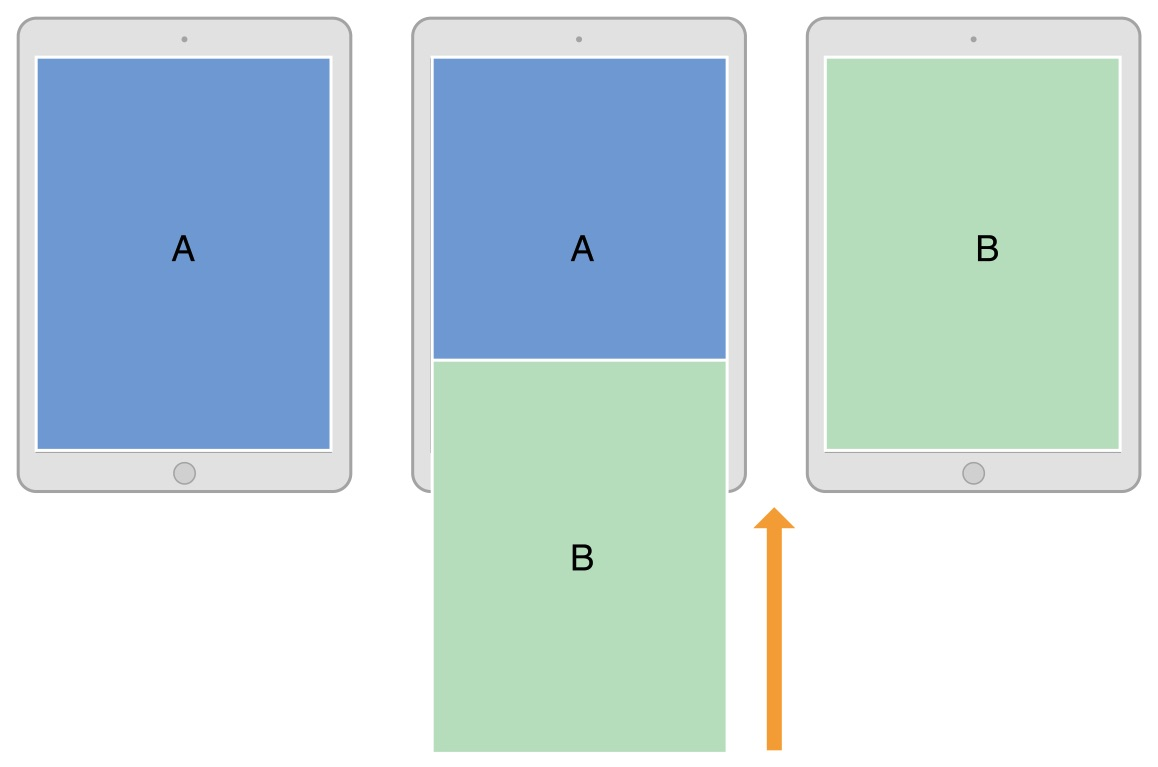
\includegraphics[width=10cm]{modal}
            \captionof{figure}{
                Presantazione di un ViewController tramite modal
            }
            \label{fig:3}
        \end{minipage}
    }
    \item{\textbf{Segue}: Una segue non è altro che un link tra due view controller attraverso un'interfaccia
        grafica. In base alla tipologia cambia il tipo di navigazione (Modal o Push). Le segue vengono utilizzate programmaticamente o nei file \textbf{storyboard}, in cui
        ogni ViewController viene "disegnato", e poi linkato ad altri ViewController.
    }
\end{enumerate}

\section{UIKit Dynamics}

Per la progettazione iniziale delle animazioni è stato fatto un attento studio a delle metodologie e dei frameworks
atti a creare animazioni interattive fluide.

Alla fine è stato deciso di utilizzare un pacchetto
nativo di iOS incluso nello UIKit\cite{uikit}, chiamato UIKit Dynamics\cite{uidynamics}: questo framework,
con una serie di API, offre delle funzioni di animazione base che 
donano alle viste i comportamenti fisici del mondo reale.

Il framework si basa su degli oggetti \textbf{UIDynamicAnimator} in cui ogni animator è responsabile delle
animazioni che avvengono sulla sua \textbf{referenceView} e si inizializza 
attraverso la seguente funzione:

\begin{minted}{swift}
    UIDynamicAnimator.init(referenceView view: UIView)
\end{minted}

% una volta inizializzato attraverso la funzione addBehavior sarà posibile assegnargli
% dei comportamenti fisici predefiniti.

\subsection{Comportamenti base}

Definiamo \textbf{DynamicItem} qualsiasi vista a cui viene assegnato un \textbf{UIDynamicBehavior}.
Ogni animator attraverso il metodo addBehavior può assegnare a determinate
viste comportamenti fisici elencati di seguito: 

\begin{itemize}
    % \item\textbf{UIDynamicBehavior}: il comportamento base da cui ereditano tutti gli altri;
    \item\textbf{UIAttachmentBehavior}: crea una relazione o legame tra due DynamicItem o tra un DynamicItem e un punto di ancoraggio;
    \item\textbf{UICollisionBehavior}: un oggetto che conferisce a un array di DynamicItems la possibilità di impegnarsi in collisioni tra loro e con i limiti specificati del comportamento;
    \item\textbf{UIFieldBehavior}: un oggetto che conferisce delle proprietà magnetiche e elettriche a un DynamicItem;
    \item\textbf{UIGravityBehavior}: aggiunge all'oggetto un forza di gravità;
    \item\textbf{UIPushBehavior}: aggiunge all'oggetto una forza continua o istantanea in una direzione specifica;
    \item\textbf{UISnapBehavior}: un comportamento simile a una molla il cui movimento iniziale viene smorzato nel tempo in modo che l'oggetto si stabilizzi in un punto specifico.
\end{itemize}

Un esempio di implementazione degli strumenti UIDynamics in QIX e mostrato in figura~\ref{fig:6}

\begin{minipage}{\linewidth}
    \centering
    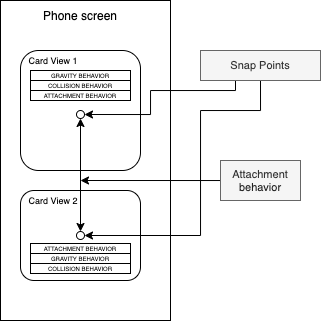
\includegraphics[width=10cm]{animation}
    \captionof{figure}{
       Schema dell'implementazione di UIDynamics
    }
    \label{fig:6}
\end{minipage}\\\\

\section{UIWindow}\label{sec:uiwindow}

Il contenuto di ogni applicazione iOS è inserito all'interno di un oggetto denominato
\textbf{UIWindow}\cite{uiwindow}. Questa finestra è disponibile in ogni UIViewController e permette di aggiungere contenuti
come viste o interi UIViewController al di sopra di tutto il contesto dell'app. Questo rende essenzialmente ogni contenuto presentato
indipendente per esempio da uno stack di navigazione.

\begin{minipage}{\linewidth}
    \centering
    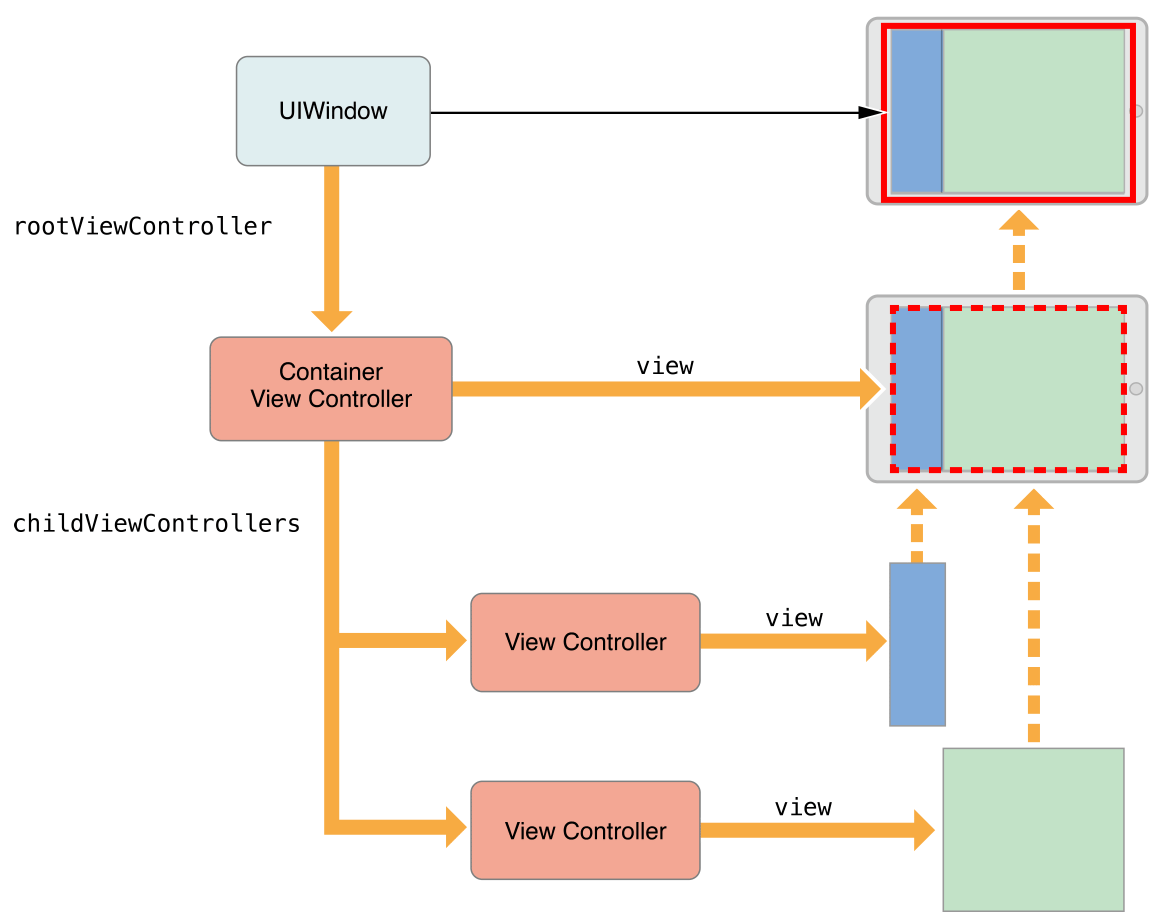
\includegraphics[width=8cm]{uiwindow}
    \captionof{figure}{Rappresentazione dell UIWindow}
    \label{fig:7}
\end{minipage}\\


\section{Delegation pattern}\label{delegation}

Il \textbf{Delegation pattern} è uno dei pattern più usati nelle app iOS. In particolare in QIX
è stato molto sfruttato per la comunicazione tra ViewController e Coordinator.

Tale pattern non è altro che un insieme di interfacce e metodi che
vengono progettate per pubblicizzare con il resto dell'applicazione degli eventi che avvengono in uno specifico ViewController.

In \textbf{Swift} le interfaccie si utilizzano attraverso la Keyword \textbf{protocol}. Questi oggetti possono contenere metodi, variabili, closure
e sono molto utili per la definizione di strutture dinamiche tipizzate.

Swift è un linguaggio di programmazione Object Oriented utilizzato per la creazione di applicazioni per dispositivi Apple. È un
linguaggio molto innovativo creato da Apple nel 2014, ad oggi siamo alla versione 5.1 e negli anni ha subito molti cambiamenti e evoluzioni.

\subsection{Esempio Delegation}

Un semplice esempio potrebbe essere un ViewController che vuole
pubblicizzare la pressione di un buttone e dall'altra parte il coordinator
che viene notificato e agirà di conseguenza:

\begin{minted}{swift}

// ------------- View controller -------------
// Interfaccia per la definizione delle API
protocol ExampleViewControllerDelegate {
    func exampleViewController(_ controller: UIViewController,
        didPressButton button: Any)
}

class ExampleViewController: UIViewController {

    // Istanza opzionale del delegate
    weak var delegate: ExampleViewControllerDelegate?

    // Evento di pressione del bottone
    @IBAction func buttonPressed(_ sender: Any) {
        // Se istanziato il delegate lancia la funzione
        self.delegate?.exampleViewController(self,
            didPressButton: sender)
    }
}

// ------------- Coordinator -------------
class ExampleCoordinator: Coordinator {

    private var exampleViewController: ExampleViewController

    func init() {
        let exampleViewController = ExampleViewController()
        self.exampleViewController = exampleViewController

        // Presentazione modale dell'exampleViewController
        self.present(exampleViewController, animated: true)
    }

    func start() {
        // Impostazione del delegate
        exampleViewController.delegate = self
        // ...
    }
}

extension ParentViewController: ExampleViewControllerDelegate {
    func exampleViewController(_ controller: UIViewController,
        didPressButton button: Any){
        
        // Handling della pressione del bottone
    }
}
\end{minted}

Nell'esempio è in parte utilizzato anche il Coordinator Pattern che spiegherò al capitolo~\ref{CH:3}.

\section{UIGestureRecognizer}

In iOS per interagire con le viste attraverso il display touch screen si utilizzano delle UIGestureRecognizer.
Tali strumenti sono nativi e ne esistono diverse tipologie in base al tipo di interazione con l'utente:

\begin{itemize}
    \item UITapGestureRecognizer: responsabile della gestione dei tap

    \item UIPinchGestureRecognizer: responsabile della gestione del pinch ossia la gesture spesso usata per lo zoom
    
    \item UIRotationGestureRecognizer: responsabile della gestione delle rotazioni
    
    \item UISwipeGestureRecognizer: responsabile di uno swipe ossia un trascinamento molto breve in una direzione 
    
    \item UIPanGestureRecognizer: responsabile del drag and drop
    
    \item UIScreenEdgePanGestureRecognizer: responsabile di una Pan gesture localizzata ai limiti destro e sinistro dello schermo
    
    \item UILongPressGestureRecognizer: responsabile di una pressione di tocco prolungata nel tempo e maggiore di un valore di soglia
\end{itemize}

In QIX è stata usata una UIPanGestureRecognizer per la gestione del trascinamento delle CardView animate.
L'implementazione è mostrata nella sezione~\ref{gestureimplemention}